\section{Durchführung}
\label{sec:durchführung}

Zur Herstellung von Debye-Scherrer Aufnahmen müssen zunächst die Proben präpariert werden. Dazu wird ein im Durchmesser
etwa $\SI{1}{\milli\meter}$ messender, kleiner Glaszylinder zur Fixierung des kristallinen Pulvers eingefettet.
Die Salze werden zunächst um maximale Feinheit zu erreichen in einem Mörser zerstoßen. Anschließend wird das Pulver
auf den Zylinder aufgetragen. Die Probe wird in der Mitte der Kamera fixiert und mit Hilfe einer Justierschraube möglichst
mittig und stabil ausgerichtet. Bevor die Probe der Röntgenstrahlung ausgesetzt wird, muss das Innere der Kamera
noch mit einem Fotofilm ausgekleidet werden. Hierbei sind zwei Löcher im Film nötig, durch welche die Strahlung
eintreten und gestoppt werden kann. Die so präparierte Probe wird dann in die Röntgenquelle eingeführt und über einen
Elektromotor kontinuierlich gedreht. Eine schematische Darstellung liegt in Abbildung~\ref{fig:aufbau} vor.
Über 2 bzw. 3 Stunden wird die Probe so der Strahlung ausgesetzt und der Film anschließend in der Dunkelkammer entwickelt. \\
Dieses Verfahren wird für ein Salz und eine metallische Verbindung durchgeführt.
%
\begin{figure}[htb]
  \centering
  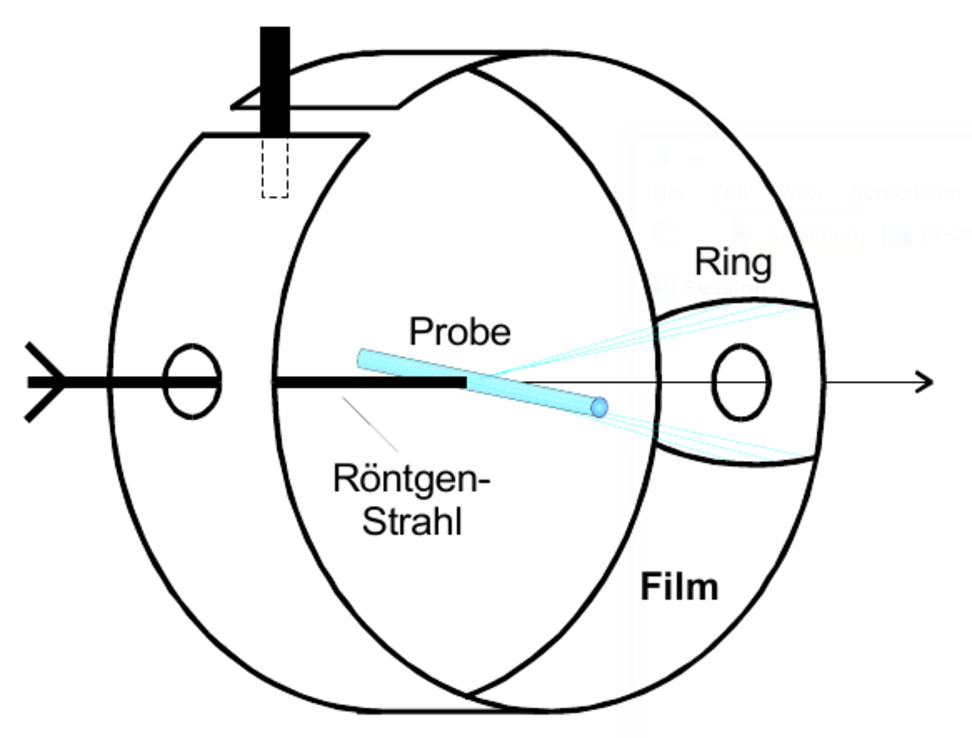
\includegraphics[width=0.7\textwidth]{figures/plot_aufbau.pdf}
  \caption{Schematischer Aufbau der Kamera. Die Probe befindet sich in der Mitte der Kamera und ist außen umgeben von dem Fotofilm \cite{V41}.}
  \label{fig:aufbau}
\end{figure}
